\capitulo{5}{Aspectos relevantes del desarrollo del proyecto}

En este apartado se van a recoger los aspectos más importantes que han surgido en el desarrollo del proyecto. Se incluirán la toma de decisiones, los posibles cambios, la aparición de problemas y las soluciones establecidas.

\section{Inicio del proyecto}\label{inicio_del_proyecto}

Al principio se propuso la idea de la creación de un Sistema de Información (\emph{Data Ware-House} o almacén de datos), para almacenar información relevante para la matriculación de alumnos en la Universidad de Burgos (UBU) y su futura utilización para la toma de decisiones.

Por esta razón, la idea transmitida por el tutor fue la creación de un sistema para poder almacenar y visualizar cualquier grado o máster de la UBU.

El tutor comentó que los archivos que se iban a utilizar de partida, eran un tipo de ficheros descargado desde una aplicación denominada \emph{Sigma} y tenían un error de formato.

Con este conjunto de ideas y proposiciones, se realizaron los \emph{Objetivos del proyecto} y se enviaron al tutor para la supervisión de los mismos.

Tras la aprobación o visto bueno, se empieza a realizar el proyecto, con la creación del repositorio en \emph{GitHub} el día 26 de febrero de 2019.

%\imagenflotante{logo}{Logotipo del Sistema de Información sobre Matriculación}

\begin{figure}%[!h]
		\centering
		
\includegraphics[width=0.5\textwidth]{logo}
		\caption{Logotipo del Sistema de Información sobre Matriculación}\label{fig:logo}
\end{figure}

 
\section{Metodologías}\label{metodologias}

A lo largo del desarrollo del proyecto se ha usado la \emph{metodología Scrum}. Se trata de una metodología ágil basada en \emph{sprints}, en este caso, de desarrollo incremental con revisiones semanales.

Por lo tanto, la duración estimada de cada \emph{sprint} es de una semana, si bien ha habido varios \emph{sprints} que han tenido una duración superior. Al finalizar cada \emph{sprint}, se planificaba el siguiente, creando sus \emph{issues} o tareas a realizar en dicho \emph{sprint}. Cuando estas tareas se realizaban, se cambiaba el estado del \emph{issue} correspondiente a \emph{Closed} o cerrado.  


\section{Toma de decisiones}\label{toma_de_decisiones}


\section{Librerías para el tratamiento y manipulación de datos}\label{librerias}
En este apartado se van a explicar las diferentes librerías o bibliotecas que se han utilizado en el desarrollo del proyecto y su función principal. Todas las librerías explicadas a continuación son de \emph{Python}.

\subsection{re}
La primera librería que se ha utilizado en el proyecto ha sido re\footnote{\href {https://docs.python.org/3/library/re.html}{www.docs.python.org/3/library/re}}, ya que dicha librería contiene las funciones necesarias para trabajar con expresiones regulares.

Las expresiones regulares se han utilizado sobretodo en la parte inicial de parsear los ficheros descargados de Sigma. De esta manera se ha podido separar y extraer información por filas, celdas y contenido de las mismas.


\subsection{pandas}
Pandas\footnote{\href{https://pandas.pydata.org/}{www.pandas.pydata.org}} es una librería que ofrece numerosas estructuras de datos de gran rendimiento y herramientas de análisis de datos.

Esta librería se ha utilizado principalmente para abrir y crear archivos con \emph{Python} y para crear \emph{dataframes} o estructuras auxiliares donde guardar datos.  


\subsection{sqlite3}
Como ya se ha comentado en un apartado anterior, la librería sqlite3\footnote{\href{https://docs.python.org/2/library/sqlite3.html}{www.docs.python.org/2/library/sqlite3.html}} proporciona una base de datos relacional de pequeño tamaño, ya que no necesita un servidor para poder utilizarse, ya que los datos se almacenan en un único fichero en el sistema host.

Esta librería se ha utilizado para la creación de la base de datos(BBDD), así como para la carga de datos y los procesos de consultas a la misma.

\subsection{Tkinter}
Tkinter\footnote{\href{https://docs.python.org/2/library/tkinter.html}{www.docs.python.org/2/library/tkinter.html}} es una librería con numerosas funciones para hacer posible la creación de una interfaz gráfica en \emph{Python}.

Se trata de una librería orientada a objetos y gracias a su facilidad de uso y rapidez para realizar una GUI, es una de las librerías más destacadas de este lenguaje de programación.

Por lo tanto, se ha utilizado principalmente en la creación de la interfaz gráfica(botones, desplegables, ventanas nuevas...etc).


\subsection{math}
La librería o componente math\footnote{\href{https://docs.python.org/3/library/math.html}{www.docs.python.org/3/library/math.html}} incluye principalmente funciones matemáticas, para realizan operaciones aritméticas. 


\subsection{matplotlib}
La librería matplotlib\footnote{\href{https://matplotlib.org/}{www.matplotlib.org}} cuenta con multitud de funciones y características para generar gráficos. Hay que destacar que se pueden generar una gran variedad de gráficos(de sector, de barras...), así como personalizar los mismos(ejes, etiquetas, fuente, leyenda...)

Esta librería se ha utilizado para la realización y personalización de los gráficos de la interfaz gráfica.


\subsection{os}
La librería os\footnote{\href{https://docs.python.org/3/library/os.html}{www.docs.python.org/3/library/os.html}} de Python permite poder usar funcionalidades relacionadas con el Sistema Operativo. 

Las funciones más destacadas de esta librería y las que se han utilizado son las que informan sobre el entorno del Sistema Operativo y las que permiten navegar por la estructura de directorios, ya sea para leer o modificar archivos.


\section{Interfaz de usuario del proyecto}\label{interfaz_de_usuario_del_proyecto}
Para la realización de este proyecto se ha realizado una GUI (Graphical User Interface) o interfaz de usuario para hacer más sencillo la comunicación entre el usuario y el sistema.

Se ha optado por la realización de una aplicación de escritorio, ya que era la mejor opción para el uso que se espera que se le dé en un futuro a la aplicación.



\section{Problemas encontrados}

\subsection{Error al abrir los Excel(.xls) bajados de Sigma con Python}
Los archivos Excel(.xls) suministrados (descargados de plataforma \emph{Sigma}) no cumplen el estándar. Al abrirlos tanto con Excel como con varias librerías de Python, muestran un error de formato y extensión. Por lo tanto la única solución encontrada, ha sido realizar un parseo previo de los Excel suministrados, creando un fichero (.csv) nuevo, con toda la información del fichero original corrupto.

De esta manera, se ha creado un analizador sintáctico capaz de leer los ficheros originales (.xls) en modo texto (.xml) y finalmente obtener un (.csv). Se ha parseado toda la información obteniendo filas, celdas, separaciones entre las mismas, contenidos de cada celda...etc. A la vez que se extrae toda esta información, se crea un fichero (.csv) nuevo y se van introduciendo los datos.

También se ha decidido modificar el fichero (.csv) resultante, añadiendo una nueva columna al final del encabezado principal de los datos. Esta nueva columna se ha llamado \emph{Plan} y de esta manera, se evita tener que estar volviendo a introducir cada encabezado de datos(repetido) por cada diferente Plan o Titulación que se incluya en el fichero (.xls).


\begin{figure}%[!h]
	\centering
	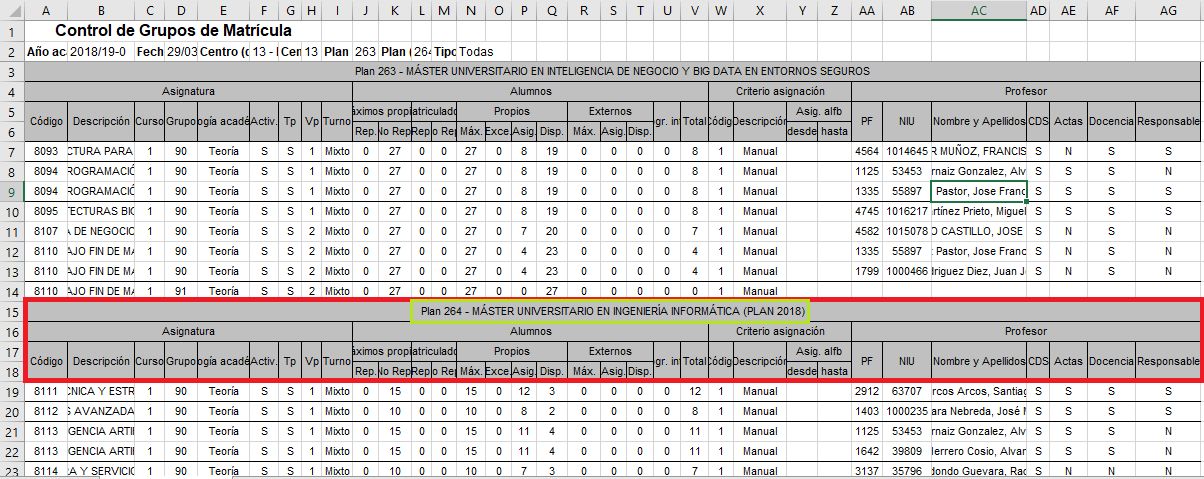
\includegraphics[angle=90, width=0.6\textwidth]{datosFicheroOriginalRojo}
	\caption{Datos del fichero original}\label{fig:datosFicheroOriginalRojo}
\end{figure}

%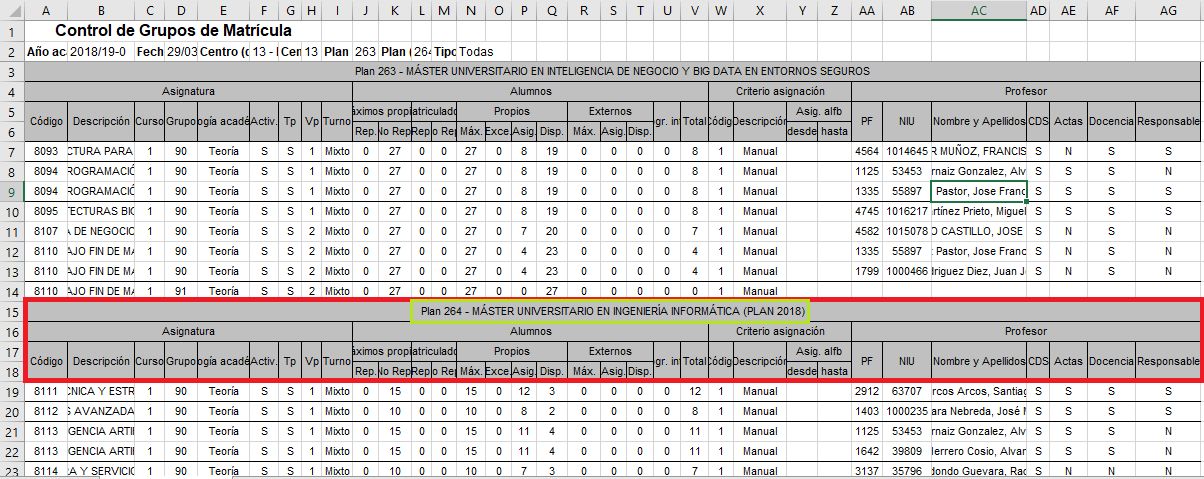
\includegraphics[angle=90, scale = 0.60]{datosFicheroOriginalRojo}
%\imagen{datosFicheroOriginalRojo}{Datos del fichero original}

De esta manera, obtenemos:


\begin{figure}%[!h]
	\centering
	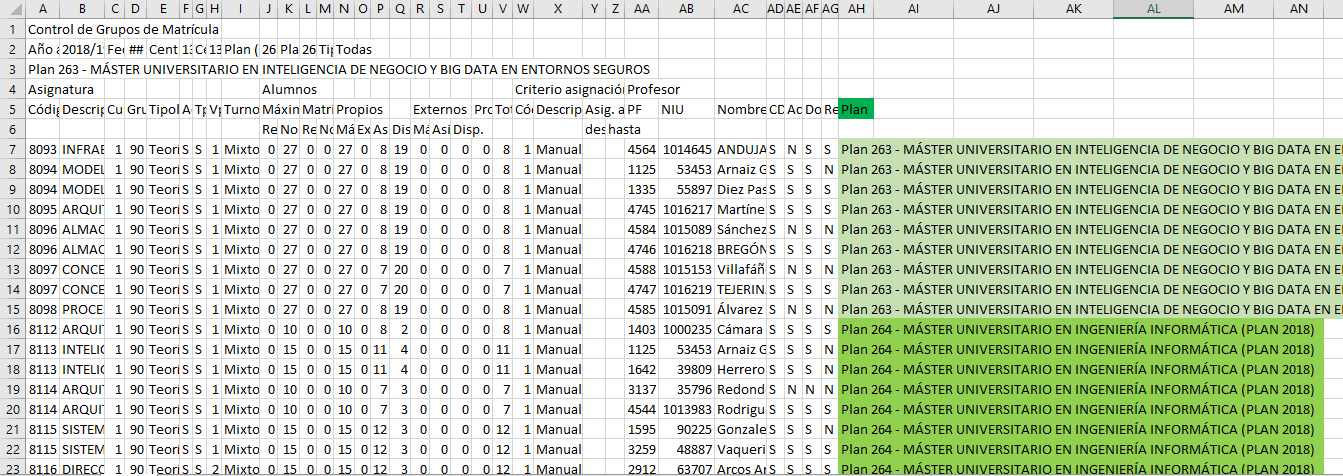
\includegraphics[angle=90, width=0.6\textwidth]{datosFicheroCSVColumnaAnadida}
	\caption{Datos del fichero parseado con columna añadida}\label{fig:datosFicheroCSVColumnaAnadida}
\end{figure}

%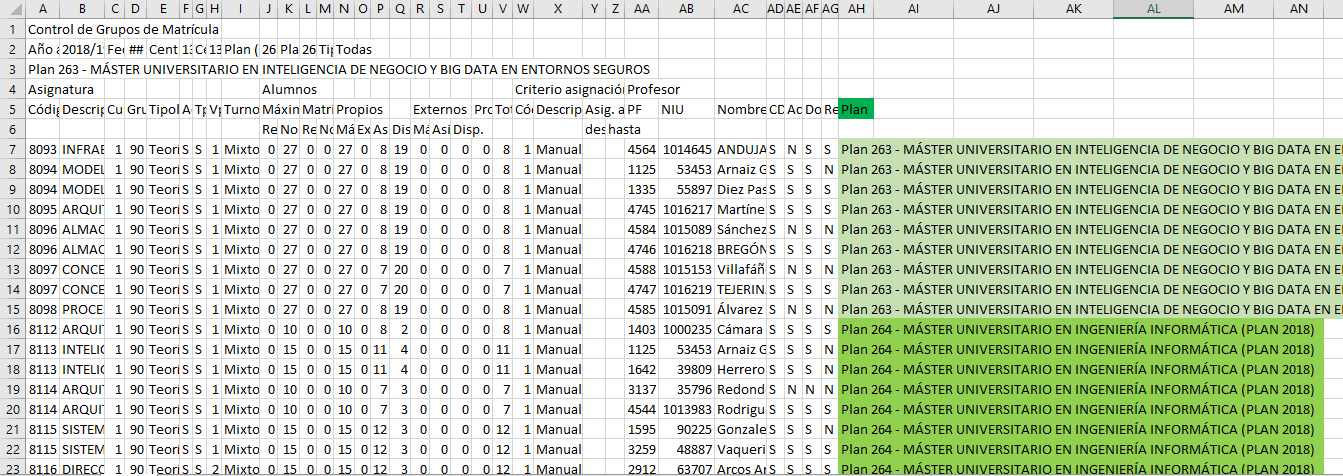
\includegraphics[angle=90, scale = 0.60]{datosFicheroCSVColumnaAnadida}
%\imagen{datosFicheroCSVColumnaAnadida}{Datos del fichero parseado con columna añadida}



En un primer lugar no se esperaba que estos ficheros fueran a generar muchos problemas, ya que al tratarse de una hoja de cálculo de Excel con extensión (.xls), al abrir los ficheros con dicho programa, se mostraba una pantalla de error, indicando el siguiente tipo de error, el cual el propio programa era capaz de solucionar, pudiendo visualizar todos los datos contenidos en el archivo:


\begin{figure}%[!h]
	\centering
	
\includegraphics[ width=\textwidth]{errorFicheroOriginal}
	\caption{Error al intentar abrir con Excel los ficheros originales}\label{fig:errorFicheroOriginal}
\end{figure}

%
\includegraphics[ scale = 0.60]{errorFicheroOriginal}
%\imagen{errorFicheroOriginal}{Error al intentar abrir con Excel los ficheros originales}

Como se conseguía ver el contenido de los ficheros, así como su formato(color de celdas, celdas unificadas...); se pensó que podría ser un pequeño problema. Realmente se apreció la dimensión del problema cuando se intentó importar y abrir los datos con librerías específicas de \emph{Python} como \emph{Pandas}.

Al comprobar que no se podía cargar u obtener la información de de ninguna manera, se optó por crear un analizador sintáctico o parser para realizar un parseo de los datos. De esta manera se abría el fichero (.xls) como si fuera un fichero de texto, con lo cual obteníamos un fichero (.xml) para analizar. Tras analizar y parsear este último fichero, se obtenía toda la información del (.xls) original(ROW, CELL, MergeDown, MergeAcross, DATA...) y con esta información se creaba un fichero resultante (.csv). 

Más adelante se optó por eliminar las cabeceras repetidas en el caso de tener más de una Titulación o Plan en un mismo fichero(recuadro en rojo de la imagen x).


Como en las cabeceras, la información del Plan (recuadro verde de la imagen x) no se debía perder, se añadió una nueva columna(imagen y) para almacenar esa información de las cabeceras repetidas que se iban a prescindir.




De esta manera se obtubo un fichero (.csv) final mejor estructurado y preparado para hacer más eficiente la carga de datos a la BBDD.


  

